\chapter{Исследовательский раздел}
В данном разделе представлены технические характеристики компьютера, используемого для тестирования и экспериментов, и результат работы программы.
 \section{Технические характеристики}

Ниже приведены технические характеристики устройства, на котором были проведены эксперименты при помощи разработанного ПО:

\begin{itemize}
	\item операционная система: Windows 10 (64-разрядная);
	\item оперативная память: 32 GB;
	\item процессор: Intel(R) Core(TM) i7-7700K CPU @ 4.20GHz;
	\item количество ядер: 4;
	\item количество потоков: 8.
\end{itemize}

\section{Результат рыботы программы}
На рисунке \ref{results} представлены результаты работы программы для обработки 10 заявок, каждая из которых содержит строку из 10000 слов, состоящих из 1-10 букв.

\begin{figure}[h]
	\center{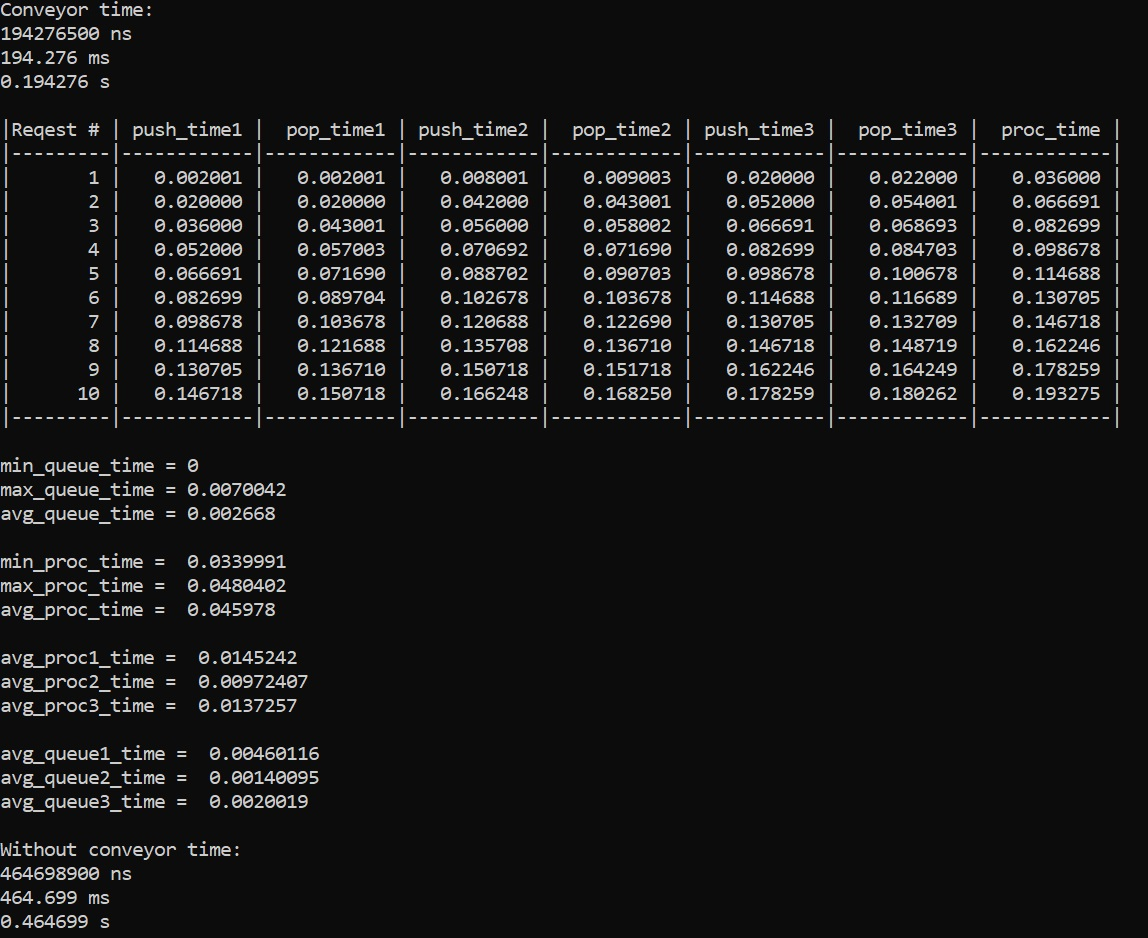
\includegraphics[width=1\linewidth]{inc/img/results}}
	\caption{Результат работы программы}
	\label{results}
\end{figure}

\newpage
Из результатов следует, что больше всего  времени в среднем тратится на разбиение строки на слова (1-я лента конвейера), меньше всего -- на поиск полиндромов среди них (2-я лента конвейера
%, 2-я стадия обработки данных
). Соответственно, время простоя в первой очереди --- наибольшее, а во второй --- наименьшее. Также, реализация с конвейером быстрее справилась с заявками, чем реализация с последовательной обработкой.

!! либо русские буквы в примере, либо нужны комментарии к обзначениям на рисунке

\section{Вывод}
По итогу иследования выяснилось, что разработанный алгоритм работает верно, то есть находит самый длинный полиндром в строке. Кроме этого был проведён анализ и сделан вывод по логу программы.